\newcommand{\NWtarget}[2]{#2}
\newcommand{\NWlink}[2]{#2}
\newcommand{\NWtxtMacroDefBy}{Fragment defined by}
\newcommand{\NWtxtMacroRefIn}{Fragment referenced in}
\newcommand{\NWtxtMacroNoRef}{Fragment never referenced}
\newcommand{\NWtxtDefBy}{Defined by}
\newcommand{\NWtxtRefIn}{Referenced in}
\newcommand{\NWtxtNoRef}{Not referenced}
\newcommand{\NWtxtFileDefBy}{File defined by}
\newcommand{\NWtxtIdentsUsed}{Uses:}
\newcommand{\NWtxtIdentsNotUsed}{Never used}
\newcommand{\NWtxtIdentsDefed}{Defines:}
\newcommand{\NWsep}{${\diamond}$}
\newcommand{\NWnotglobal}{(not defined globally)}
\newcommand{\NWuseHyperlinks}{}
\documentclass[12pt]{article}
\usepackage{graphicx}
\usepackage{amssymb}
\usepackage{listings}
\usepackage{amsmath}
\usepackage{graphicx}
\usepackage{float}
\usepackage[section]{placeins}
% Russian specicfic
% -------------------------
\usepackage[T2A]{fontenc}
\usepackage[utf8]{inputenc}
\usepackage[russian]{babel}
% -------------------------

\graphicspath{{./figs/}}

\begin{document}

\title{Общая связность сети. Критическое ребро.}

\author{
  Кирпа Вадим
  \and
  Махлярчук Андрей
  \and
  Утин Никита
  \and
  Березкин Аркадий
%  \and
%  Блинов Игорь
}

\maketitle
\thispagestyle{empty}
\newpage

\section{Постановка задачи:}

\paragraph{}
Для графа $G = (V, E, W)$ с множеством вершин $V$,
множеством ребер $W: E \rightarrow \mathbb{R}_+$
найти ребро $e^*$, такое, что при замене
$W(e^*) \rightarrow \gamma W(e^*)$ сумма сетевых 
расстояний между всеми узлами минимизируется
(при $\gamma < 1$) или максимизируется (при $\gamma > 1$).
Расчеты привести для графа Владивостока-2012.

\section{Алгоритм}

\paragraph{}
Для нахождения суммы сетевых расстояний в графе использовался
алгоритм Дейкстры\cite{dijkstra}.

\paragraph{}
Чтобы найти критическое ребро сумма сетевых расстояний считается
для всех подграфов $G_i$, где $W(e_i) \rightarrow \gamma W(e_i)$. Если сумма сетевых
ребер в текущем подграфе $G_i$ меньше (больше при $\gamma > 1$)
ранее найденой суммы, то это ребро сохраняется в качестве претендента
на критическое. В конце работы алгоритма мы получаем критическое ребро, 
сумму сетевых расстояний, соответствующую графу с обновленным весом критического ребра и новый вес данного ребра.

\section{Реализация} 
В начале выполнения программы происходит считывание графа из файла. 
Затем для каждой вершины запускаем алгоритм Дейкстры. В данной рализации можно было бы использовать 
алгоритм Флойда-Уоршелла, но было принято решение реализовать алгоритм Дейкстры, так как он легче поддается распараллеливанию.

\paragraph{}
Алгоритм реализован на языке C++. Основной процедурой является
алгоритм Дейкстры\cite{dijkstra}.


\subsection{Исходный код}
\paragraph{}
Ниже приведен код класса описывающего ребро графа.
\begin{flushleft} \small
\begin{minipage}{\linewidth}\label{scrap1}\raggedright\small
\NWtarget{nuweb3}{} \verb@"src/edge.h"@\nobreak\ {\footnotesize {3}}$\equiv$
\vspace{-1ex}
\begin{list}{}{} \item
\mbox{}\verb@@\\
\mbox{}\verb@#pragma once@\\
\mbox{}\verb@#include <atomic>@\\
\mbox{}\verb@#include <functional>@\\
\mbox{}\verb@@\\
\mbox{}\verb@class Edge {@\\
\mbox{}\verb@public:@\\
\mbox{}\verb@    @\hbox{$\langle\,${\itshape constructors}\nobreak\ {\footnotesize \NWlink{nuweb4a}{4a}}$\,\rangle$}\verb@@\\
\mbox{}\verb@    @\hbox{$\langle\,${\itshape getters and setters}\nobreak\ {\footnotesize \NWlink{nuweb4b}{4b}}$\,\rangle$}\verb@@\\
\mbox{}\verb@private:@\\
\mbox{}\verb@    int left;@\\
\mbox{}\verb@    int right;@\\
\mbox{}\verb@    double weight;@\\
\mbox{}\verb@    int id;@\\
\mbox{}\verb@};@\\
\mbox{}\verb@@\\
\mbox{}\verb@@\hbox{$\langle\,${\itshape utilities}\nobreak\ {\footnotesize \NWlink{nuweb5a}{5a}}$\,\rangle$}\verb@@\\
\mbox{}\verb@@\\
\mbox{}\verb@@{\NWsep}
\end{list}
\vspace{-1.5ex}
\footnotesize
\begin{list}{}{\setlength{\itemsep}{-\parsep}\setlength{\itemindent}{-\leftmargin}}

\item{}
\end{list}
\end{minipage}\vspace{4ex}
\end{flushleft}
\paragraph{}
Класс имеет 2 конструктора, один из которых конструктор копирования.
Конструктор мринимает 2 номера соеденяемых вершин типа $int$, 
вес ребра типа $double$ и уникальный $id$ типа, для того чтобы 
можно было эффективно искать ребра. Эти данные сохраняются в качестве
полей объекта. 

\begin{flushleft} \small
\begin{minipage}{\linewidth}\label{scrap2}\raggedright\small
\NWtarget{nuweb4a}{} $\langle\,${\itshape constructors}\nobreak\ {\footnotesize {4a}}$\,\rangle\equiv$
\vspace{-1ex}
\begin{list}{}{} \item
\mbox{}\verb@@\\
\mbox{}\verb@Edge(const Edge& e) :@\\
\mbox{}\verb@    left(e.left), @\\
\mbox{}\verb@    right(e.right), @\\
\mbox{}\verb@    weight(e.weight), @\\
\mbox{}\verb@    id(e.id) { }@\\
\mbox{}\verb@Edge(int u, int v, double w, int id) : @\\
\mbox{}\verb@    left(u), @\\
\mbox{}\verb@    right(v), @\\
\mbox{}\verb@    weight(w), @\\
\mbox{}\verb@    id(id) { }@\\
\mbox{}\verb@@{\NWsep}
\end{list}
\vspace{-1.5ex}
\footnotesize
\begin{list}{}{\setlength{\itemsep}{-\parsep}\setlength{\itemindent}{-\leftmargin}}
\item \NWtxtMacroRefIn\ \NWlink{nuweb3}{3}.

\item{}
\end{list}
\end{minipage}\vspace{4ex}
\end{flushleft}
\paragraph{}
Класс имеет геттеры для всех полей объектов и сеттер для поля $weight$, т.к.
необходимо динамически изменять вес ребер в графе, чтобы пересчитывать суммы сетевых расстояний.

\begin{flushleft} \small
\begin{minipage}{\linewidth}\label{scrap3}\raggedright\small
\NWtarget{nuweb4b}{} $\langle\,${\itshape getters and setters}\nobreak\ {\footnotesize {4b}}$\,\rangle\equiv$
\vspace{-1ex}
\begin{list}{}{} \item
\mbox{}\verb@@\\
\mbox{}\verb@const int GetLeft() const { return left; }@\\
\mbox{}\verb@const int GetRight() const { return right; }@\\
\mbox{}\verb@const double GetWeight() const { return weight; }@\\
\mbox{}\verb@const int getId() const { return id; }@\\
\mbox{}\verb@void SetWeight(double w) { weight = w; }@\\
\mbox{}\verb@@{\NWsep}
\end{list}
\vspace{-1.5ex}
\footnotesize
\begin{list}{}{\setlength{\itemsep}{-\parsep}\setlength{\itemindent}{-\leftmargin}}
\item \NWtxtMacroRefIn\ \NWlink{nuweb3}{3}.

\item{}
\end{list}
\end{minipage}\vspace{4ex}
\end{flushleft}
\paragraph{}
Для удобства использования струкрутры были написаны операторы.

\begin{flushleft} \small
\begin{minipage}{\linewidth}\label{scrap4}\raggedright\small
\NWtarget{nuweb5a}{} $\langle\,${\itshape utilities}\nobreak\ {\footnotesize {5a}}$\,\rangle\equiv$
\vspace{-1ex}
\begin{list}{}{} \item
\mbox{}\verb@@\\
\mbox{}\verb@struct EdgeHash {@\\
\mbox{}\verb@    unsigned int operator()(const Edge& e) const {@\\
\mbox{}\verb@        return std::hash<int>()(e.GetRight());@\\
\mbox{}\verb@    }@\\
\mbox{}\verb@};@\\
\mbox{}\verb@@\\
\mbox{}\verb@bool operator==(const Edge& e, const Edge& t);@\\
\mbox{}\verb@@{\NWsep}
\end{list}
\vspace{-1.5ex}
\footnotesize
\begin{list}{}{\setlength{\itemsep}{-\parsep}\setlength{\itemindent}{-\leftmargin}}
\item \NWtxtMacroRefIn\ \NWlink{nuweb3}{3}.

\item{}
\end{list}
\end{minipage}\vspace{4ex}
\end{flushleft}
\begin{flushleft} \small
\begin{minipage}{\linewidth}\label{scrap5}\raggedright\small
\NWtarget{nuweb5b}{} \verb@"src/edge.cpp"@\nobreak\ {\footnotesize {5b}}$\equiv$
\vspace{-1ex}
\begin{list}{}{} \item
\mbox{}\verb@@\\
\mbox{}\verb@#include "edge.h"@\\
\mbox{}\verb@@\\
\mbox{}\verb@bool operator==(const Edge& e, const Edge& t) {@\\
\mbox{}\verb@    return e.GetRight() == t.GetRight();@\\
\mbox{}\verb@}@\\
\mbox{}\verb@@{\NWsep}
\end{list}
\vspace{-1.5ex}
\footnotesize
\begin{list}{}{\setlength{\itemsep}{-\parsep}\setlength{\itemindent}{-\leftmargin}}

\item{}
\end{list}
\end{minipage}\vspace{4ex}
\end{flushleft}
\paragraph{}
Код класса описывающий граф.

\begin{flushleft} \small
\begin{minipage}{\linewidth}\label{scrap6}\raggedright\small
\NWtarget{nuweb6}{} \verb@"src/graph.h"@\nobreak\ {\footnotesize {6}}$\equiv$
\vspace{-1ex}
\begin{list}{}{} \item
\mbox{}\verb@@\\
\mbox{}\verb@@\hbox{$\langle\,${\itshape includes}\nobreak\ {\footnotesize \NWlink{nuweb7a}{7a}}$\,\rangle$}\verb@@\\
\mbox{}\verb@class Graph {@\\
\mbox{}\verb@public:@\\
\mbox{}\verb@    @\hbox{$\langle\,${\itshape graph constructors}\nobreak\ {\footnotesize \NWlink{nuweb7b}{7b}}$\,\rangle$}\verb@@\\
\mbox{}\verb@    @\hbox{$\langle\,${\itshape graph edges}\nobreak\ {\footnotesize \NWlink{nuweb8a}{8a}}$\,\rangle$}\verb@@\\
\mbox{}\verb@    @\hbox{$\langle\,${\itshape graph open}\nobreak\ {\footnotesize \NWlink{nuweb8b}{8b}}$\,\rangle$}\verb@@\\
\mbox{}\verb@    @\hbox{$\langle\,${\itshape graph dijkstra}\nobreak\ {\footnotesize \NWlink{nuweb8c}{8c}}$\,\rangle$}\verb@@\\
\mbox{}\verb@    @\hbox{$\langle\,${\itshape graph find critical}\nobreak\ {\footnotesize \NWlink{nuweb8d}{8d}}$\,\rangle$}\verb@@\\
\mbox{}\verb@private:@\\
\mbox{}\verb@    @\hbox{$\langle\,${\itshape graph inf}\nobreak\ {\footnotesize \NWlink{nuweb9a}{9a}}$\,\rangle$}\verb@@\\
\mbox{}\verb@    @\hbox{$\langle\,${\itshape graph data}\nobreak\ {\footnotesize \NWlink{nuweb9b}{9b}}$\,\rangle$}\verb@@\\
\mbox{}\verb@    @\hbox{$\langle\,${\itshape graph used}\nobreak\ {\footnotesize \NWlink{nuweb9c}{9c}}$\,\rangle$}\verb@@\\
\mbox{}\verb@    @\hbox{$\langle\,${\itshape graph distsum}\nobreak\ {\footnotesize \NWlink{nuweb10a}{10a}}$\,\rangle$}\verb@@\\
\mbox{}\verb@    @\hbox{$\langle\,${\itshape graph dijkstra2}\nobreak\ {\footnotesize \NWlink{nuweb10b}{10b}}$\,\rangle$}\verb@@\\
\mbox{}\verb@    @\hbox{$\langle\,${\itshape graph run dijkstra}\nobreak\ {\footnotesize \NWlink{nuweb10c}{10c}}$\,\rangle$}\verb@@\\
\mbox{}\verb@    @\hbox{$\langle\,${\itshape graph add edge}\nobreak\ {\footnotesize \NWlink{nuweb10d}{10d}}$\,\rangle$}\verb@@\\
\mbox{}\verb@};@\\
\mbox{}\verb@@\\
\mbox{}\verb@    @\hbox{$\langle\,${\itshape graph operator}\nobreak\ {\footnotesize \NWlink{nuweb11a}{11a}}$\,\rangle$}\verb@@\\
\mbox{}\verb@@{\NWsep}
\end{list}
\vspace{-1.5ex}
\footnotesize
\begin{list}{}{\setlength{\itemsep}{-\parsep}\setlength{\itemindent}{-\leftmargin}}

\item{}
\end{list}
\end{minipage}\vspace{4ex}
\end{flushleft}
\paragraph{}
Зависимости класса описывающего граф.

\begin{flushleft} \small
\begin{minipage}{\linewidth}\label{scrap7}\raggedright\small
\NWtarget{nuweb7a}{} $\langle\,${\itshape includes}\nobreak\ {\footnotesize {7a}}$\,\rangle\equiv$
\vspace{-1ex}
\begin{list}{}{} \item
\mbox{}\verb@@\\
\mbox{}\verb@#pragma once@\\
\mbox{}\verb@#include <unordered_map>@\\
\mbox{}\verb@#include <unordered_set>@\\
\mbox{}\verb@#include <set>@\\
\mbox{}\verb@#include <iostream>@\\
\mbox{}\verb@#include <fstream>@\\
\mbox{}\verb@#include <queue>@\\
\mbox{}\verb@#include <string>@\\
\mbox{}\verb@#include <atomic>@\\
\mbox{}\verb@#include <thread>@\\
\mbox{}\verb@#include <sstream>@\\
\mbox{}\verb@#include <regex>@\\
\mbox{}\verb@#include "edge.h"@\\
\mbox{}\verb@#include <cfloat>@\\
\mbox{}\verb@@\\
\mbox{}\verb@@{\NWsep}
\end{list}
\vspace{-1.5ex}
\footnotesize
\begin{list}{}{\setlength{\itemsep}{-\parsep}\setlength{\itemindent}{-\leftmargin}}
\item \NWtxtMacroRefIn\ \NWlink{nuweb6}{6}.

\item{}
\end{list}
\end{minipage}\vspace{4ex}
\end{flushleft}
\paragraph{}
Конструкторы класса описывающего граф.

\begin{flushleft} \small
\begin{minipage}{\linewidth}\label{scrap8}\raggedright\small
\NWtarget{nuweb7b}{} $\langle\,${\itshape graph constructors}\nobreak\ {\footnotesize {7b}}$\,\rangle\equiv$
\vspace{-1ex}
\begin{list}{}{} \item
\mbox{}\verb@@\\
\mbox{}\verb@Graph();@\\
\mbox{}\verb@Graph(std::string filename);@\\
\mbox{}\verb@@{\NWsep}
\end{list}
\vspace{-1.5ex}
\footnotesize
\begin{list}{}{\setlength{\itemsep}{-\parsep}\setlength{\itemindent}{-\leftmargin}}
\item \NWtxtMacroRefIn\ \NWlink{nuweb6}{6}.

\item{}
\end{list}
\end{minipage}\vspace{4ex}
\end{flushleft}
\paragraph{}
Поле для хранения ребер графа. Для эффективности вычислений используется std::unordered_map. 

\begin{flushleft} \small
\begin{minipage}{\linewidth}\label{scrap9}\raggedright\small
\NWtarget{nuweb8a}{} $\langle\,${\itshape graph edges}\nobreak\ {\footnotesize {8a}}$\,\rangle\equiv$
\vspace{-1ex}
\begin{list}{}{} \item
\mbox{}\verb@@\\
\mbox{}\verb@std::unordered_map <int, std::unordered_set <Edge, EdgeHash>> edges;@\\
\mbox{}\verb@@{\NWsep}
\end{list}
\vspace{-1.5ex}
\footnotesize
\begin{list}{}{\setlength{\itemsep}{-\parsep}\setlength{\itemindent}{-\leftmargin}}
\item \NWtxtMacroRefIn\ \NWlink{nuweb6}{6}.

\item{}
\end{list}
\end{minipage}\vspace{4ex}
\end{flushleft}
\paragraph{}
Функция для считывания графа из файла.

\begin{flushleft} \small
\begin{minipage}{\linewidth}\label{scrap10}\raggedright\small
\NWtarget{nuweb8b}{} $\langle\,${\itshape graph open}\nobreak\ {\footnotesize {8b}}$\,\rangle\equiv$
\vspace{-1ex}
\begin{list}{}{} \item
\mbox{}\verb@@\\
\mbox{}\verb@void open(std::string filename);@\\
\mbox{}\verb@@{\NWsep}
\end{list}
\vspace{-1.5ex}
\footnotesize
\begin{list}{}{\setlength{\itemsep}{-\parsep}\setlength{\itemindent}{-\leftmargin}}
\item \NWtxtMacroRefIn\ \NWlink{nuweb6}{6}.

\item{}
\end{list}
\end{minipage}\vspace{4ex}
\end{flushleft}
\paragraph{}
Функция,запускающая алгоритм Дейкстры в разных потоках.
\begin{flushleft} \small
\begin{minipage}{\linewidth}\label{scrap11}\raggedright\small
\NWtarget{nuweb8c}{} $\langle\,${\itshape graph dijkstra}\nobreak\ {\footnotesize {8c}}$\,\rangle\equiv$
\vspace{-1ex}
\begin{list}{}{} \item
\mbox{}\verb@@\\
\mbox{}\verb@double RunDijkstraAsync();    @\\
\mbox{}\verb@@{\NWsep}
\end{list}
\vspace{-1.5ex}
\footnotesize
\begin{list}{}{\setlength{\itemsep}{-\parsep}\setlength{\itemindent}{-\leftmargin}}
\item \NWtxtMacroRefIn\ \NWlink{nuweb6}{6}.

\item{}
\end{list}
\end{minipage}\vspace{4ex}
\end{flushleft}
\paragraph{}
Основная функция, осуществляющая поиск критического ребра в исходном графе. В качестве аргумента принимает значение $\gamma$
из исходной задачи.
\begin{flushleft} \small
\begin{minipage}{\linewidth}\label{scrap12}\raggedright\small
\NWtarget{nuweb8d}{} $\langle\,${\itshape graph find critical}\nobreak\ {\footnotesize {8d}}$\,\rangle\equiv$
\vspace{-1ex}
\begin{list}{}{} \item
\mbox{}\verb@@\\
\mbox{}\verb@void FindCriticalEdge(double k);@\\
\mbox{}\verb@@{\NWsep}
\end{list}
\vspace{-1.5ex}
\footnotesize
\begin{list}{}{\setlength{\itemsep}{-\parsep}\setlength{\itemindent}{-\leftmargin}}
\item \NWtxtMacroRefIn\ \NWlink{nuweb6}{6}.

\item{}
\end{list}
\end{minipage}\vspace{4ex}
\end{flushleft}
\paragraph{}
Константа имтирующая бесконечность в поиске путей алгоритмом Дейкстры.
\begin{flushleft} \small
\begin{minipage}{\linewidth}\label{scrap13}\raggedright\small
\NWtarget{nuweb9a}{} $\langle\,${\itshape graph inf}\nobreak\ {\footnotesize {9a}}$\,\rangle\equiv$
\vspace{-1ex}
\begin{list}{}{} \item
\mbox{}\verb@@\\
\mbox{}\verb@static const long long inf = std::numeric_limits<long long>::max();@\\
\mbox{}\verb@@{\NWsep}
\end{list}
\vspace{-1.5ex}
\footnotesize
\begin{list}{}{\setlength{\itemsep}{-\parsep}\setlength{\itemindent}{-\leftmargin}}
\item \NWtxtMacroRefIn\ \NWlink{nuweb6}{6}.

\item{}
\end{list}
\end{minipage}\vspace{4ex}
\end{flushleft}
\paragraph{}
Поля необходимые для хранения перенумерованных вершин графа.

\begin{flushleft} \small
\begin{minipage}{\linewidth}\label{scrap14}\raggedright\small
\NWtarget{nuweb9b}{} $\langle\,${\itshape graph data}\nobreak\ {\footnotesize {9b}}$\,\rangle\equiv$
\vspace{-1ex}
\begin{list}{}{} \item
\mbox{}\verb@@\\
\mbox{}\verb@std::unordered_map<int, int> coord;@\\
\mbox{}\verb@std::unordered_map<int, int> coord_to_vertecies;@\\
\mbox{}\verb@@{\NWsep}
\end{list}
\vspace{-1.5ex}
\footnotesize
\begin{list}{}{\setlength{\itemsep}{-\parsep}\setlength{\itemindent}{-\leftmargin}}
\item \NWtxtMacroRefIn\ \NWlink{nuweb6}{6}.

\item{}
\end{list}
\end{minipage}\vspace{4ex}
\end{flushleft}
\paragraph{}
Структура данных, сохраняющая индексы использованных ребер. 
\begin{flushleft} \small
\begin{minipage}{\linewidth}\label{scrap15}\raggedright\small
\NWtarget{nuweb9c}{} $\langle\,${\itshape graph used}\nobreak\ {\footnotesize {9c}}$\,\rangle\equiv$
\vspace{-1ex}
\begin{list}{}{} \item
\mbox{}\verb@@\\
\mbox{}\verb@std::unordered_set<int> usedEdges;@\\
\mbox{}\verb@@{\NWsep}
\end{list}
\vspace{-1.5ex}
\footnotesize
\begin{list}{}{\setlength{\itemsep}{-\parsep}\setlength{\itemindent}{-\leftmargin}}
\item \NWtxtMacroRefIn\ \NWlink{nuweb6}{6}.

\item{}
\end{list}
\end{minipage}\vspace{4ex}
\end{flushleft}
\paragraph{}
Массив необходимый для хранения сетевых расстояний, получаемых алгоритмом Дейкстры, запущенным в разных потоках. 
\begin{flushleft} \small
\begin{minipage}{\linewidth}\label{scrap16}\raggedright\small
\NWtarget{nuweb10a}{} $\langle\,${\itshape graph distsum}\nobreak\ {\footnotesize {10a}}$\,\rangle\equiv$
\vspace{-1ex}
\begin{list}{}{} \item
\mbox{}\verb@@\\
\mbox{}\verb@std::vector<double> distSum;@\\
\mbox{}\verb@@{\NWsep}
\end{list}
\vspace{-1.5ex}
\footnotesize
\begin{list}{}{\setlength{\itemsep}{-\parsep}\setlength{\itemindent}{-\leftmargin}}
\item \NWtxtMacroRefIn\ \NWlink{nuweb6}{6}.

\item{}
\end{list}
\end{minipage}\vspace{4ex}
\end{flushleft}
\paragraph{}
Функция реализующая алгоритм Дейкстры. Принимает на вход номер вершины.
\begin{flushleft} \small
\begin{minipage}{\linewidth}\label{scrap17}\raggedright\small
\NWtarget{nuweb10b}{} $\langle\,${\itshape graph dijkstra2}\nobreak\ {\footnotesize {10b}}$\,\rangle\equiv$
\vspace{-1ex}
\begin{list}{}{} \item
\mbox{}\verb@@\\
\mbox{}\verb@double Dijkstra(int v);@\\
\mbox{}\verb@@{\NWsep}
\end{list}
\vspace{-1.5ex}
\footnotesize
\begin{list}{}{\setlength{\itemsep}{-\parsep}\setlength{\itemindent}{-\leftmargin}}
\item \NWtxtMacroRefIn\ \NWlink{nuweb6}{6}.

\item{}
\end{list}
\end{minipage}\vspace{4ex}
\end{flushleft}
\paragraph{}
Функция запускающая алгоритм дейкстры $Dijkstra(int v)$.
\begin{flushleft} \small
\begin{minipage}{\linewidth}\label{scrap18}\raggedright\small
\NWtarget{nuweb10c}{} $\langle\,${\itshape graph run dijkstra}\nobreak\ {\footnotesize {10c}}$\,\rangle\equiv$
\vspace{-1ex}
\begin{list}{}{} \item
\mbox{}\verb@@\\
\mbox{}\verb@void RunDijkstraThread(int from, int len);@\\
\mbox{}\verb@@{\NWsep}
\end{list}
\vspace{-1.5ex}
\footnotesize
\begin{list}{}{\setlength{\itemsep}{-\parsep}\setlength{\itemindent}{-\leftmargin}}
\item \NWtxtMacroRefIn\ \NWlink{nuweb6}{6}.

\item{}
\end{list}
\end{minipage}\vspace{4ex}
\end{flushleft}
\paragraph{}
Функция, добавляющая ребро в граф. Принимает на вход номера вершин, вес, индекс нового ребра.
\begin{flushleft} \small
\begin{minipage}{\linewidth}\label{scrap19}\raggedright\small
\NWtarget{nuweb10d}{} $\langle\,${\itshape graph add edge}\nobreak\ {\footnotesize {10d}}$\,\rangle\equiv$
\vspace{-1ex}
\begin{list}{}{} \item
\mbox{}\verb@@\\
\mbox{}\verb@void AddEdge(int index, int vertex, double weight, int id);   @\\
\mbox{}\verb@@{\NWsep}
\end{list}
\vspace{-1.5ex}
\footnotesize
\begin{list}{}{\setlength{\itemsep}{-\parsep}\setlength{\itemindent}{-\leftmargin}}
\item \NWtxtMacroRefIn\ \NWlink{nuweb6}{6}.

\item{}
\end{list}
\end{minipage}\vspace{4ex}
\end{flushleft}
\paragraph{}
Для удобства сравнения объектов класса перегружен слудющий оператор.
\begin{flushleft} \small
\begin{minipage}{\linewidth}\label{scrap20}\raggedright\small
\NWtarget{nuweb11a}{} $\langle\,${\itshape graph operator}\nobreak\ {\footnotesize {11a}}$\,\rangle\equiv$
\vspace{-1ex}
\begin{list}{}{} \item
\mbox{}\verb@@\\
\mbox{}\verb@class Compare {@\\
\mbox{}\verb@public:@\\
\mbox{}\verb@    bool operator()(std::pair<double, int> a, std::pair<double, int> b) {@\\
\mbox{}\verb@        return a.first > b.first;@\\
\mbox{}\verb@    }@\\
\mbox{}\verb@};@\\
\mbox{}\verb@@{\NWsep}
\end{list}
\vspace{-1.5ex}
\footnotesize
\begin{list}{}{\setlength{\itemsep}{-\parsep}\setlength{\itemindent}{-\leftmargin}}
\item \NWtxtMacroRefIn\ \NWlink{nuweb6}{6}.

\item{}
\end{list}
\end{minipage}\vspace{4ex}
\end{flushleft}
Ниже приведена реализация фукнций описанного выше класса в $graph.h$

\begin{flushleft} \small\label{scrap21}\raggedright\small
\NWtarget{nuweb11b}{} \verb@"src/graph.cpp"@\nobreak\ {\footnotesize {11b}}$\equiv$
\vspace{-1ex}
\begin{list}{}{} \item
\mbox{}\verb@@\\
\mbox{}\verb@#include <vector>@\\
\mbox{}\verb@#include "graph.h"@\\
\mbox{}\verb@@\\
\mbox{}\verb@using namespace std;@\\
\mbox{}\verb@@\\
\mbox{}\verb@//Public methods@\\
\mbox{}\verb@@\\
\mbox{}\verb@Graph::Graph() { }@\\
\mbox{}\verb@@\\
\mbox{}\verb@Graph::Graph(std::string filename) {@\\
\mbox{}\verb@    open(filename);@\\
\mbox{}\verb@}@\\
\mbox{}\verb@@\\
\mbox{}\verb@void Graph::open(std::string filename) {@\\
\mbox{}\verb@    if (filename != "") {@\\
\mbox{}\verb@        std::ifstream in(filename);@\\
\mbox{}\verb@        int index, vertex;@\\
\mbox{}\verb@        double weight;@\\
\mbox{}\verb@        int n = 0;@\\
\mbox{}\verb@        int id = 0;@\\
\mbox{}\verb@        while (!in.eof()) {@\\
\mbox{}\verb@            int v;@\\
\mbox{}\verb@            int u;@\\
\mbox{}\verb@            in >> index >> vertex >> weight;@\\
\mbox{}\verb@            if (coord.find(index) != coord.end()) {@\\
\mbox{}\verb@                v = coord[index];@\\
\mbox{}\verb@            }@\\
\mbox{}\verb@            else {@\\
\mbox{}\verb@                v = n++;@\\
\mbox{}\verb@                coord.insert(std::make_pair(index, v));@\\
\mbox{}\verb@            }@\\
\mbox{}\verb@            if (coord.find(vertex) != coord.end()) {@\\
\mbox{}\verb@                u = coord[vertex];@\\
\mbox{}\verb@            }@\\
\mbox{}\verb@            else {@\\
\mbox{}\verb@                u = n++;@\\
\mbox{}\verb@                coord.insert(std::make_pair(vertex, u));@\\
\mbox{}\verb@            }@\\
\mbox{}\verb@            AddEdge(u, v, weight, id++);@\\
\mbox{}\verb@            AddEdge(v, u, weight, id++);@\\
\mbox{}\verb@        }@\\
\mbox{}\verb@@\\
\mbox{}\verb@        for (auto &i : coord)@\\
\mbox{}\verb@            coord_to_vertecies[i.second] = i.first;@\\
\mbox{}\verb@    }@\\
\mbox{}\verb@    distSum.resize(edges.size(), 0);@\\
\mbox{}\verb@}@\\
\mbox{}\verb@@\\
\mbox{}\verb@double Graph::RunDijkstraAsync() {@\\
\mbox{}\verb@    int threads_count = 8; //todo replace@\\
\mbox{}\verb@@\\
\mbox{}\verb@    std::vector<thread> threads;@\\
\mbox{}\verb@    int batch = edges.size() / threads_count;@\\
\mbox{}\verb@    int remainder = edges.size() % threads_count;@\\
\mbox{}\verb@    for (int i = 0; i < threads_count - 1; ++i)@\\
\mbox{}\verb@        threads.push_back(thread(@\\
\mbox{}\verb@          &Graph::RunDijkstraThread, @\\
\mbox{}\verb@          this, @\\
\mbox{}\verb@          i * batch, @\\
\mbox{}\verb@          batch@\\
\mbox{}\verb@        ));@\\
\mbox{}\verb@    threads.push_back(thread(@\\
\mbox{}\verb@        &Graph::RunDijkstraThread, @\\
\mbox{}\verb@        this, @\\
\mbox{}\verb@        (threads_count - 1) * batch, @\\
\mbox{}\verb@        batch + remainder@\\
\mbox{}\verb@      ));@\\
\mbox{}\verb@    for (int i = 0; i < threads_count; ++i)@\\
\mbox{}\verb@        threads[i].join();@\\
\mbox{}\verb@@\\
\mbox{}\verb@    double sum = 0;@\\
\mbox{}\verb@    for (auto &i : distSum)@\\
\mbox{}\verb@        sum += i;       @\\
\mbox{}\verb@    return sum;@\\
\mbox{}\verb@}@\\
\mbox{}\verb@@\\
\mbox{}\verb@void Graph::FindCriticalEdge(double k) {@\\
\mbox{}\verb@    int criticalLeft = -1;@\\
\mbox{}\verb@    int criticalRight = -1;@\\
\mbox{}\verb@    int size = edges.size();@\\
\mbox{}\verb@    int count = 0;@\\
\mbox{}\verb@    double distances = 0;@\\
\mbox{}\verb@    if (k >= 0.0 && k <= 1.0) {@\\
\mbox{}\verb@        double min = DBL_MAX;@\\
\mbox{}\verb@        for (auto &v : edges) {@\\
\mbox{}\verb@            cout << count++ << " out of " << size << flush;@\\
\mbox{}\verb@            for (auto &edge : v.second) {@\\
\mbox{}\verb@                if (usedEdges.find(edge.getId()) == usedEdges.end()) {@\\
\mbox{}\verb@                    double PrevWeight = edge.GetWeight();@\\
\mbox{}\verb@                    auto it = edges[edge.GetRight()]@\\
\mbox{}\verb@                      .find(Edge(0, edge.GetLeft(), 0, 0));@\\
\mbox{}\verb@                    int invId = it->getId();@\\
\mbox{}\verb@                    usedEdges.insert(invId);@\\
\mbox{}\verb@                    edges[edge.GetRight()].erase(it);@\\
\mbox{}\verb@                    edges[edge.GetRight()]@\\
\mbox{}\verb@                      .insert(Edge(@\\
\mbox{}\verb@                        edge.GetRight(), @\\
\mbox{}\verb@                        edge.GetLeft(), @\\
\mbox{}\verb@                        PrevWeight*k, @\\
\mbox{}\verb@                        invId));@\\
\mbox{}\verb@                    ((Edge&)edge).SetWeight(PrevWeight*k);@\\
\mbox{}\verb@                    double sum = RunDijkstraAsync();@\\
\mbox{}\verb@                    if (min > sum) {@\\
\mbox{}\verb@                        min = sum;@\\
\mbox{}\verb@                        criticalLeft = edge.GetLeft();@\\
\mbox{}\verb@                        criticalRight = edge.GetRight();@\\
\mbox{}\verb@                    }@\\
\mbox{}\verb@                    ((Edge&)edge).SetWeight(PrevWeight);@\\
\mbox{}\verb@                    edges[edge.GetRight()]@\\
\mbox{}\verb@                      .erase(Edge(0, edge.GetLeft(), 0, 0));@\\
\mbox{}\verb@                    edges[edge.GetRight()]@\\
\mbox{}\verb@                      .insert(Edge(@\\
\mbox{}\verb@                        edge.GetRight(), @\\
\mbox{}\verb@                        edge.GetLeft(), @\\
\mbox{}\verb@                        PrevWeight, @\\
\mbox{}\verb@                        invId));@\\
\mbox{}\verb@                }@\\
\mbox{}\verb@            }@\\
\mbox{}\verb@            cout << "\r";@\\
\mbox{}\verb@        }@\\
\mbox{}\verb@        cout << endl;@\\
\mbox{}\verb@        distances = min;@\\
\mbox{}\verb@    }@\\
\mbox{}\verb@    else if (k >= 1.0) {@\\
\mbox{}\verb@        double max = 0;@\\
\mbox{}\verb@        for (auto &v : edges) {@\\
\mbox{}\verb@            cout << count++ << " out of " << size << flush;@\\
\mbox{}\verb@            for (auto &edge : v.second) {@\\
\mbox{}\verb@                if (usedEdges.find(edge.getId()) == usedEdges.end()) {@\\
\mbox{}\verb@                    double PrevWeight = edge.GetWeight();@\\
\mbox{}\verb@                    auto it = edges[edge.GetRight()]@\\
\mbox{}\verb@                      .find(Edge(0, edge.GetLeft(), 0, 0));@\\
\mbox{}\verb@                    int invId = it->getId();@\\
\mbox{}\verb@                    usedEdges.insert(invId);@\\
\mbox{}\verb@                    edges[edge.GetRight()].erase(it);@\\
\mbox{}\verb@                    edges[edge.GetRight()]@\\
\mbox{}\verb@                      .insert(Edge(@\\
\mbox{}\verb@                        edge.GetRight(), @\\
\mbox{}\verb@                        edge.GetLeft(), @\\
\mbox{}\verb@                        PrevWeight*k, @\\
\mbox{}\verb@                        invId));@\\
\mbox{}\verb@                    ((Edge&)edge).SetWeight(PrevWeight*k);@\\
\mbox{}\verb@                    double sum = RunDijkstraAsync();@\\
\mbox{}\verb@                    if (max < sum) {@\\
\mbox{}\verb@                        max = sum;@\\
\mbox{}\verb@                        criticalLeft = edge.GetLeft();@\\
\mbox{}\verb@                        criticalRight = edge.GetRight();@\\
\mbox{}\verb@                    }@\\
\mbox{}\verb@                    ((Edge&)edge).SetWeight(PrevWeight);@\\
\mbox{}\verb@                    edges[edge.GetRight()]@\\
\mbox{}\verb@                      .erase(Edge(0, edge.GetLeft(), 0, 0));@\\
\mbox{}\verb@                    edges[edge.GetRight()]@\\
\mbox{}\verb@                      .insert(Edge(@\\
\mbox{}\verb@                        edge.GetRight(), @\\
\mbox{}\verb@                        edge.GetLeft(), @\\
\mbox{}\verb@                        PrevWeight, @\\
\mbox{}\verb@                        invId));@\\
\mbox{}\verb@                }@\\
\mbox{}\verb@            }@\\
\mbox{}\verb@            cout << "\r";@\\
\mbox{}\verb@        }@\\
\mbox{}\verb@        distances = max;@\\
\mbox{}\verb@    }@\\
\mbox{}\verb@    else {@\\
\mbox{}\verb@@\\
\mbox{}\verb@    }@\\
\mbox{}\verb@    if (criticalLeft != -1 && criticalRight != -1) {@\\
\mbox{}\verb@        auto edge = edges[criticalLeft].find(Edge(0, criticalRight, 0, 0));@\\
\mbox{}\verb@        cout << "New distances: " << distances << ". With edge between ";@\\
\mbox{}\verb@        cout << coord_to_vertecies[edge->GetLeft()] @\\
\mbox{}\verb@          << " and " @\\
\mbox{}\verb@          << coord_to_vertecies[edge->GetRight()] @\\
\mbox{}\verb@          << ". Weight: " @\\
\mbox{}\verb@          << edge->GetWeight() << endl;@\\
\mbox{}\verb@    }@\\
\mbox{}\verb@}@\\
\mbox{}\verb@@\\
\mbox{}\verb@@\\
\mbox{}\verb@double Graph::Dijkstra(int v) {@\\
\mbox{}\verb@    std::vector<double> dist(edges.size(), inf);@\\
\mbox{}\verb@    std::vector<bool> visited(edges.size(), false);@\\
\mbox{}\verb@    dist[v] = 0.0;@\\
\mbox{}\verb@    std::priority_queue<@\\
\mbox{}\verb@      std::pair<double, int>, @\\
\mbox{}\verb@      std::vector<std::pair<double, int>>, @\\
\mbox{}\verb@      Compare> q;@\\
\mbox{}\verb@    visited[v] = true;@\\
\mbox{}\verb@    q.push(std::make_pair(dist[v], v));@\\
\mbox{}\verb@@\\
\mbox{}\verb@    while (!q.empty()) {@\\
\mbox{}\verb@        std::pair<double, int> from = q.top(); q.pop();@\\
\mbox{}\verb@        for (auto& edge : edges[from.second]) {@\\
\mbox{}\verb@            int to = edge.GetRight();@\\
\mbox{}\verb@            if (!visited[to]) {@\\
\mbox{}\verb@                double tmp = from.first + edge.GetWeight();@\\
\mbox{}\verb@                if (dist[to] > tmp) {@\\
\mbox{}\verb@                    dist[to] = tmp;@\\
\mbox{}\verb@                    visited[to] = true;@\\
\mbox{}\verb@                    q.push(std::make_pair(tmp, to));@\\
\mbox{}\verb@                }@\\
\mbox{}\verb@            }@\\
\mbox{}\verb@        }@\\
\mbox{}\verb@    }@\\
\mbox{}\verb@    double sum = 0;@\\
\mbox{}\verb@    for (auto &i : dist)@\\
\mbox{}\verb@        if (i != inf)@\\
\mbox{}\verb@            sum += i;@\\
\mbox{}\verb@    return sum;@\\
\mbox{}\verb@}@\\
\mbox{}\verb@@\\
\mbox{}\verb@void Graph::RunDijkstraThread(int from, int len) {@\\
\mbox{}\verb@    for (int i = from; i < from + len; ++i)@\\
\mbox{}\verb@        distSum[i] = Dijkstra(i);@\\
\mbox{}\verb@}@\\
\mbox{}\verb@@\\
\mbox{}\verb@void Graph::AddEdge(int index, int vertex, double weight, int id) {@\\
\mbox{}\verb@    edges[index].insert(Edge(index, vertex, weight, id));@\\
\mbox{}\verb@}@\\
\mbox{}\verb@@\\
\mbox{}\verb@@{\NWsep}
\end{list}
\vspace{-1.5ex}
\footnotesize
\begin{list}{}{\setlength{\itemsep}{-\parsep}\setlength{\itemindent}{-\leftmargin}}

\item{}
\end{list}
\vspace{4ex}
\end{flushleft}
\paragraph{}
Ниже приведен исходный код входной точки пограммы. 
Имя файла и значение $\gamma$ передаются в качестве
параметров интерфейса командной строки.

\begin{flushleft} \small
\begin{minipage}{\linewidth}\label{scrap22}\raggedright\small
\NWtarget{nuweb18}{} \verb@"src/main.cpp"@\nobreak\ {\footnotesize {18}}$\equiv$
\vspace{-1ex}
\begin{list}{}{} \item
\mbox{}\verb@@\\
\mbox{}\verb@#include "graph.h"@\\
\mbox{}\verb@@\\
\mbox{}\verb@using namespace std;@\\
\mbox{}\verb@@\\
\mbox{}\verb@int main(int argc, char* argv[]) {@\\
\mbox{}\verb@    cout << "Reading graph" << endl;@\\
\mbox{}\verb@    Graph graph;@\\
\mbox{}\verb@    if (argc > 1)@\\
\mbox{}\verb@        graph.open(argv[1]);@\\
\mbox{}\verb@    else@\\
\mbox{}\verb@        graph.open("little.dat");@\\
\mbox{}\verb@    cout << "Read graph successfully" << endl;@\\
\mbox{}\verb@    cout << "Counting original distances" << endl;@\\
\mbox{}\verb@    cout << "Original distances: " << graph.RunDijkstraAsync() << endl;@\\
\mbox{}\verb@    double k = 1.5;@\\
\mbox{}\verb@    if (argc > 2)@\\
\mbox{}\verb@        k = atof(argv[2]);@\\
\mbox{}\verb@    cout << "Searching critical edge" << endl;@\\
\mbox{}\verb@    graph.FindCriticalEdge(k);@\\
\mbox{}\verb@    return 0;@\\
\mbox{}\verb@}@\\
\mbox{}\verb@@{\NWsep}
\end{list}
\vspace{-1.5ex}
\footnotesize
\begin{list}{}{\setlength{\itemsep}{-\parsep}\setlength{\itemindent}{-\leftmargin}}

\item{}
\end{list}
\end{minipage}\vspace{4ex}
\end{flushleft}
\paragraph{Оценка вычислительной сложности алгоритма.}

На данном графе $G = (V, E, W)$, алгоритм Дейкстры имеет вычислительную  сложность $O(V \log V + E) $.
В нашем алгоритме на каждое изменение веса ребра, запускается алгоритм Дейкстры из каждой вершины. В результате получаем 
вычислительную сложность алгоритма $O((V \log V + E)VE)$

\paragraph{Оптимизации:}
Чтобы ускорить исполнение программы, из каждой
вершины алгоритм Дейкстры запускается в отдельном
потоке. Т.к. граф разрежен в памяти он хранится в
виде списка смежности.

\section{Результаты}

\subsection{Минимальный граф}

\paragraph{}

Рассмотрим простой пример работы алгоритма на графе с 6-ю вершинами и 5-ю ребрами
представленного на рис.~\ref{fig:min_graph_4} В данном случае мы будем минимизировать сумму сетевых расстояний и
примем $\gamma = 0.5$.

\begin{figure}[h]
    \centering
    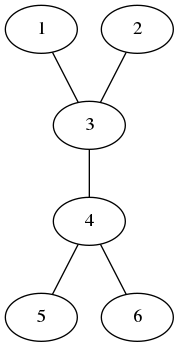
\includegraphics[scale=0.7]{min_graph_4.png}
    \caption{Минимальный граф с критическим ребром между 3-й и 4-й вершинами.}
    \label{fig:min_graph_4}
\end{figure}

Из каждой вершины исходного графа запустим алгоритм Дейкстры.
На каждом шаге работы алгоритма изменяем вес текущего ребра $W(e_i) \rightarrow \gamma W(e_i)$
Затем для данной итерации пересчитаем сумму сетевых расстояний, и, если она меньше текущей минимальной суммы,
то обновим минимум. Так в процессе работы алгоритма мы переберем все ребра и в качестве критического выберем 
ребро с соответствующей минимальной суммой сетевых расстояний. 
На каждой итерации работы алгоритма Дейкстры получим сумму сетевых расстояний для исходного графа:

\begin{gather}
1 : 1 + 5 + 6 + 6 + 2 \\
2 : 1 + 5 + 6 + 6 + 2 \\
3 : 1 + 1 + 4 + 5 + 5 \\
4 : 1 + 1 + 4 + 5 + 5 \\
5 : 1 + 5 + 6 + 6 + 2 \\
6 : 1 + 5 + 6 + 6 + 2
\end{gather}

Сумма сетевых расстояний в исходном графе $S = 112$. 

\begin{figure}[h]
    \centering
    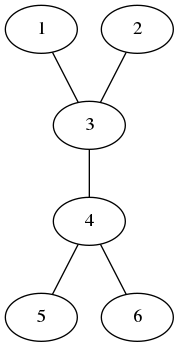
\includegraphics[scale=0.7]{min_graph_2.png}
    \caption{Если уменьшить вес ребра между 3-й и 4-й вершинами сумма сетевых расстояний минимизируется}
    \label{fig:min_graph_2}
\end{figure}

В данном граффе критическим является ребро между
3й и 4й вершинами и умножение его веса на
$\gamma < 1$ приводит к минимизации суммы сетевых расстояний.
При $\gamma = 0.5$ алгоритм меняет вес критического ребра на $0.5 \cdot w_i$ (рис.~\ref{fig:min_graph_2}).
Для обновленного графа, в котором мы заменили вес критического ребра на 2 получим сумму сетевых расстояний:

\begin{gather}
1 : 1 + 3 + 4 + 4 + 2 \\
2 : 1 + 3 + 4 + 4 + 2 \\
3 : 1 + 1 + 2 + 3 + 3 \\
4 : 1 + 1 + 2 + 3 + 3 \\
5 : 1 + 3 + 4 + 4 + 2 \\
6 : 1 + 3 + 4 + 4 + 2
\end{gather}

В таком случае сумма сетевых расстояний для обновленного графа будет равнятся $S^* = 76$.

\paragraph{При $\gamma = 2 > 1$.}
Алгоритм меняет вес критического ребра на $2 \cdot w_i = 8$ (рис.~\ref{fig:min_graph_8}).

\begin{figure}[h]
    \centering
    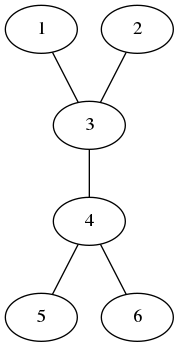
\includegraphics[scale=0.7]{min_graph_8.png}
    \caption{Если увеличить вес ребра между 3-й и 4-й вершинами сумма сетевых расстояний максимизируется}
    \label{fig:min_graph_8}
\end{figure}

В обновленном графе, с весом критического ребра = 8 мы получим следующую
сумму сетевых расстояний:

\begin{gather}
1 : 1 + 9 + 10 + 10 + 2 \\
2 : 1 + 9 + 10 + 10 + 2 \\
3 : 1 + 1 + 8  + 9  + 9 \\
4 : 1 + 1 + 8  + 9  + 9 \\
5 : 1 + 9 + 10 + 10 + 2 \\
6 : 1 + 9 + 10 + 10 + 2
\end{gather}

Что дает сумму сетевых расстояний равную $S^* = 184$

\subsection{Граф малого размера (20 вершин)}

\paragraph{}
При запуске на графе малого размера (рис~\ref{fig:small}) 
алгоритм корректно определил критическое ребро.
Этому ребру был намеренно предан большой вес для удобства тестирования.
При $k = 0.5$ и при $k = 1.5$ алгоритм определял одно
и то же ребро между 19-й и 20-й вершинами (отмечено красным),
однако изменение веса этого ребра приводило к разным итоговым
суммам сетевых расстояний, а именно к $12542$ и $14264$ соотвественно.

\begin{figure}[h]
    \centering
    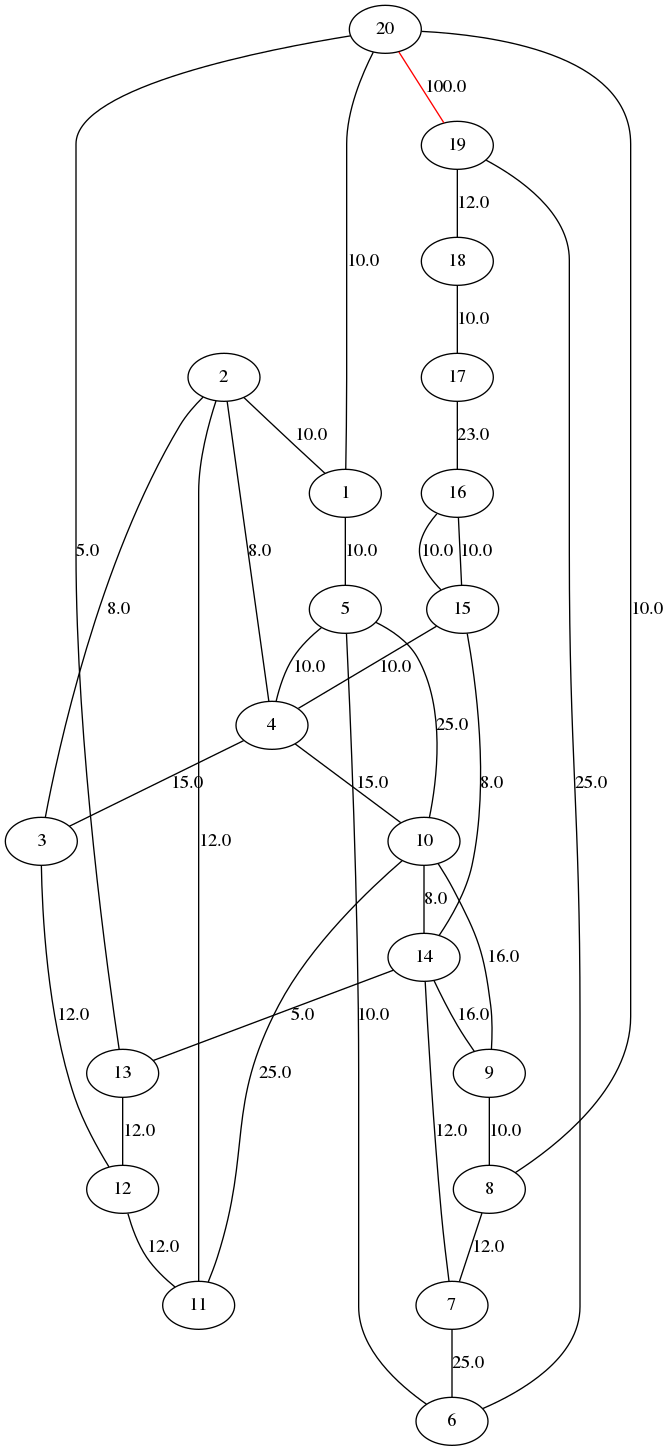
\includegraphics[scale=0.3]{small.png}
    \caption{Малый граф с 20-ю вершинами. Критическое ребро отмечено красным.}
    \label{fig:small}
\end{figure}

\subsection{Граф среднего размера (~1500 вершин)}

\paragraph{}
В качестве графа среднего размера был взят сокращеное представление 
транспортной сети города Владивостока на 2009-й годi (рис.~\ref{vlad_2009}). 
В данном представлении 1542 вершины и 1653 ребра.

\begin{figure}[h]
    \centering
    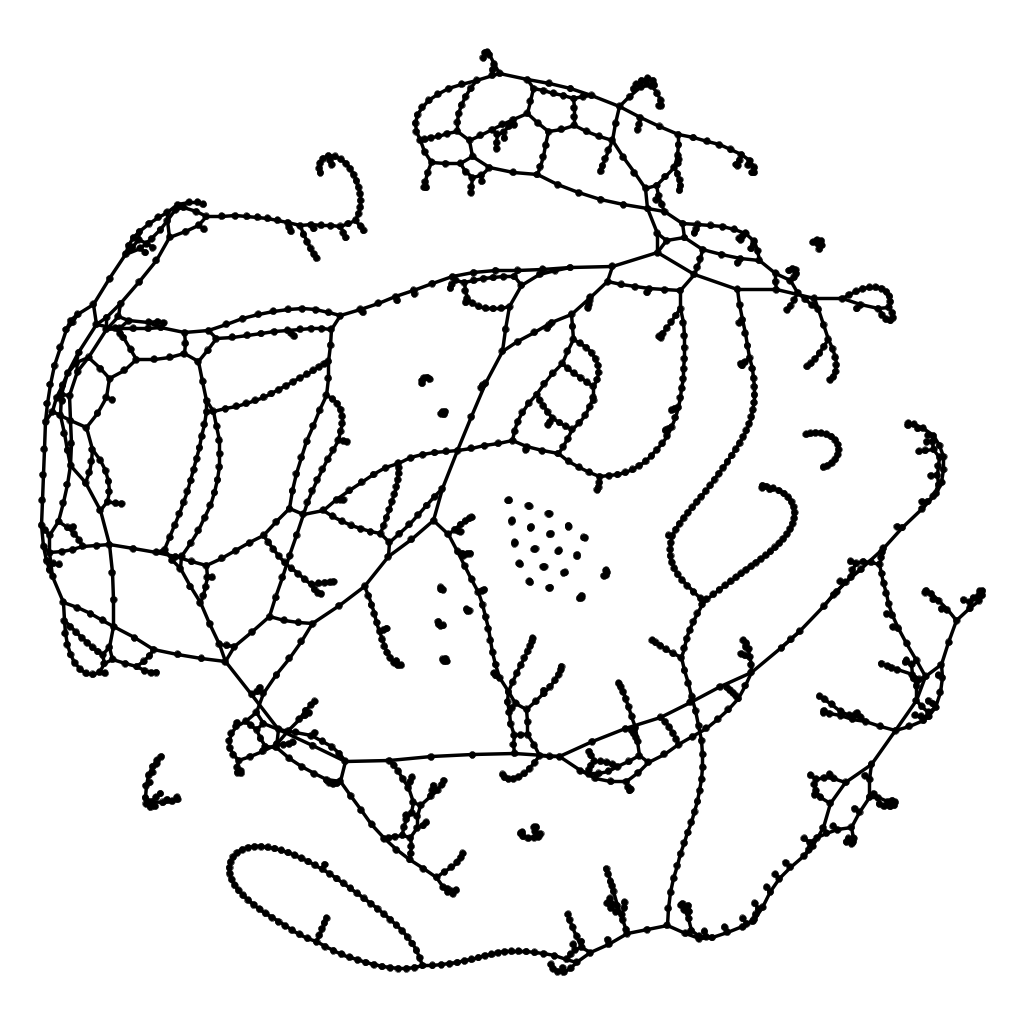
\includegraphics[scale=0.3]{vlad_2009.png}
    \caption{Сокращенная транспортная сеть города Владивостока на 2009-й год.}
    \label{fig:vlad_2009}
\end{figure}

\paragraph{}
Алгоритм был запущен с значениями $k = 0.5$ и $k = 1.5$ и определил различные
критические ребра. Ребро между

% New distances: 2.60341e+10. With edge between 175 and 176. Weight: 1008.3; k = 0.5
% New distances: 2.67274e+10. With edge between 175 and 176. Weight: 1008.3; k = 1.5

\begin{figure}[h]
    \centering
    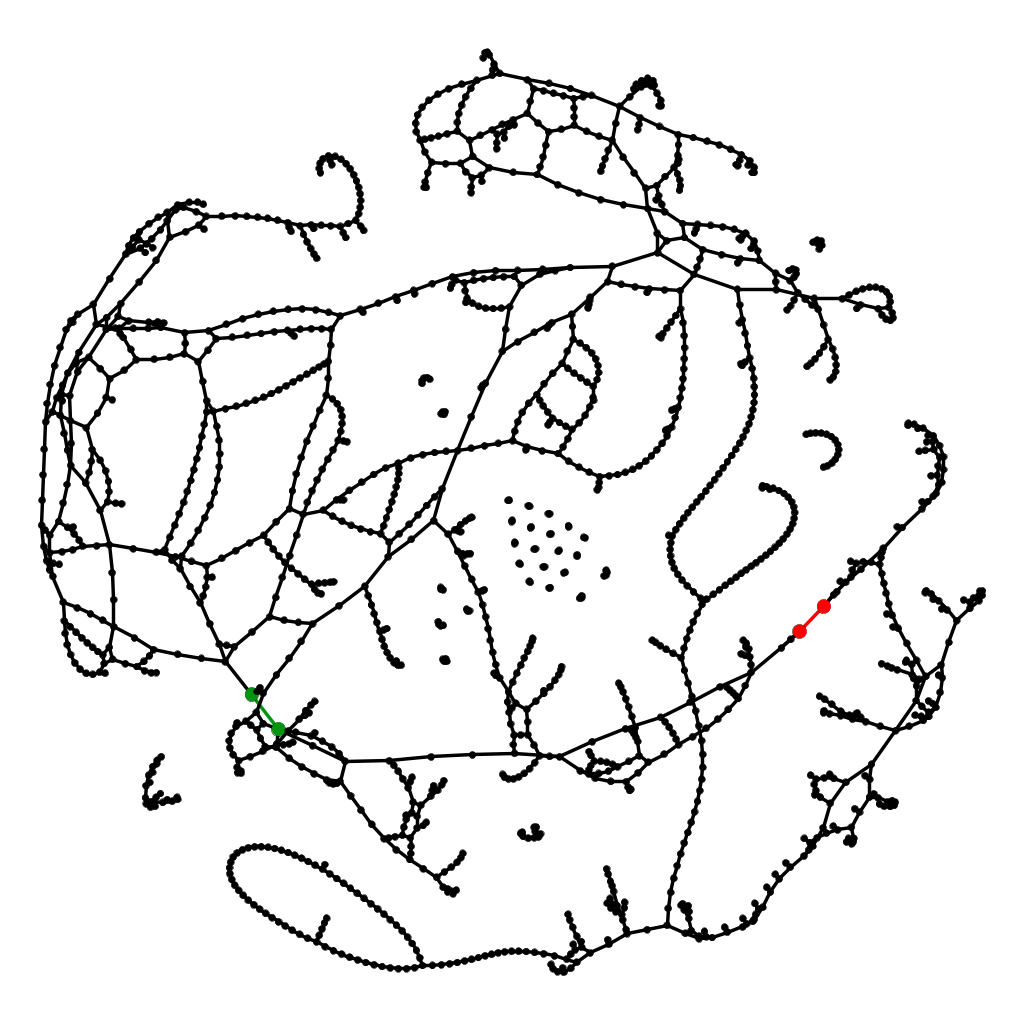
\includegraphics[scale=0.3]{vlad_2009_min_max.png}
    \caption{Сокращенная транспортная сеть города Владивостока на 2009-й год.}
    \label{fig:vlad_2009_min_max}
\end{figure}

\section{Заключение}
Окончательное и обжалованию не подлежит

\newpage

\begin{thebibliography}{9}
\bibitem{dijkstra}
Dijkstra E. W. \textit{A note on two problems in connexion with graphs} //
\textit{Numer. Math} — Springer Science+Business Media, 1959.
— Vol. 1, Iss. 1. — P. 269–271.
\end{thebibliography}

\end{document}
